\documentclass[../EDF Master Thesis.tex]{subfiles}

\begin{document}

\ac{fft} berechnet die Fourier Transformierte aus und ist ein Algorithmus der die gleichen Ergebnisse, wie die \ac{dft} liefert, jedoch mit wesentlich weniger Rechenzeit.
Dabei können beide Algorithmen ein zeitdiskretes Signal in dessen Frequenzteile (Spektrum), wie in \autoref{fig:aufspaltung_eines_Signals_in_dessen_Frequenzteile} dargestellt, aufspalten.
Dies ist sehr nützlich für viele Bereiche der Signalverarbeitung z.B. für das Komprimieren von Musikaufnahmen, wo nicht hörbare Frequenzen entfernt werden.

\begin{figure}[ht!]
    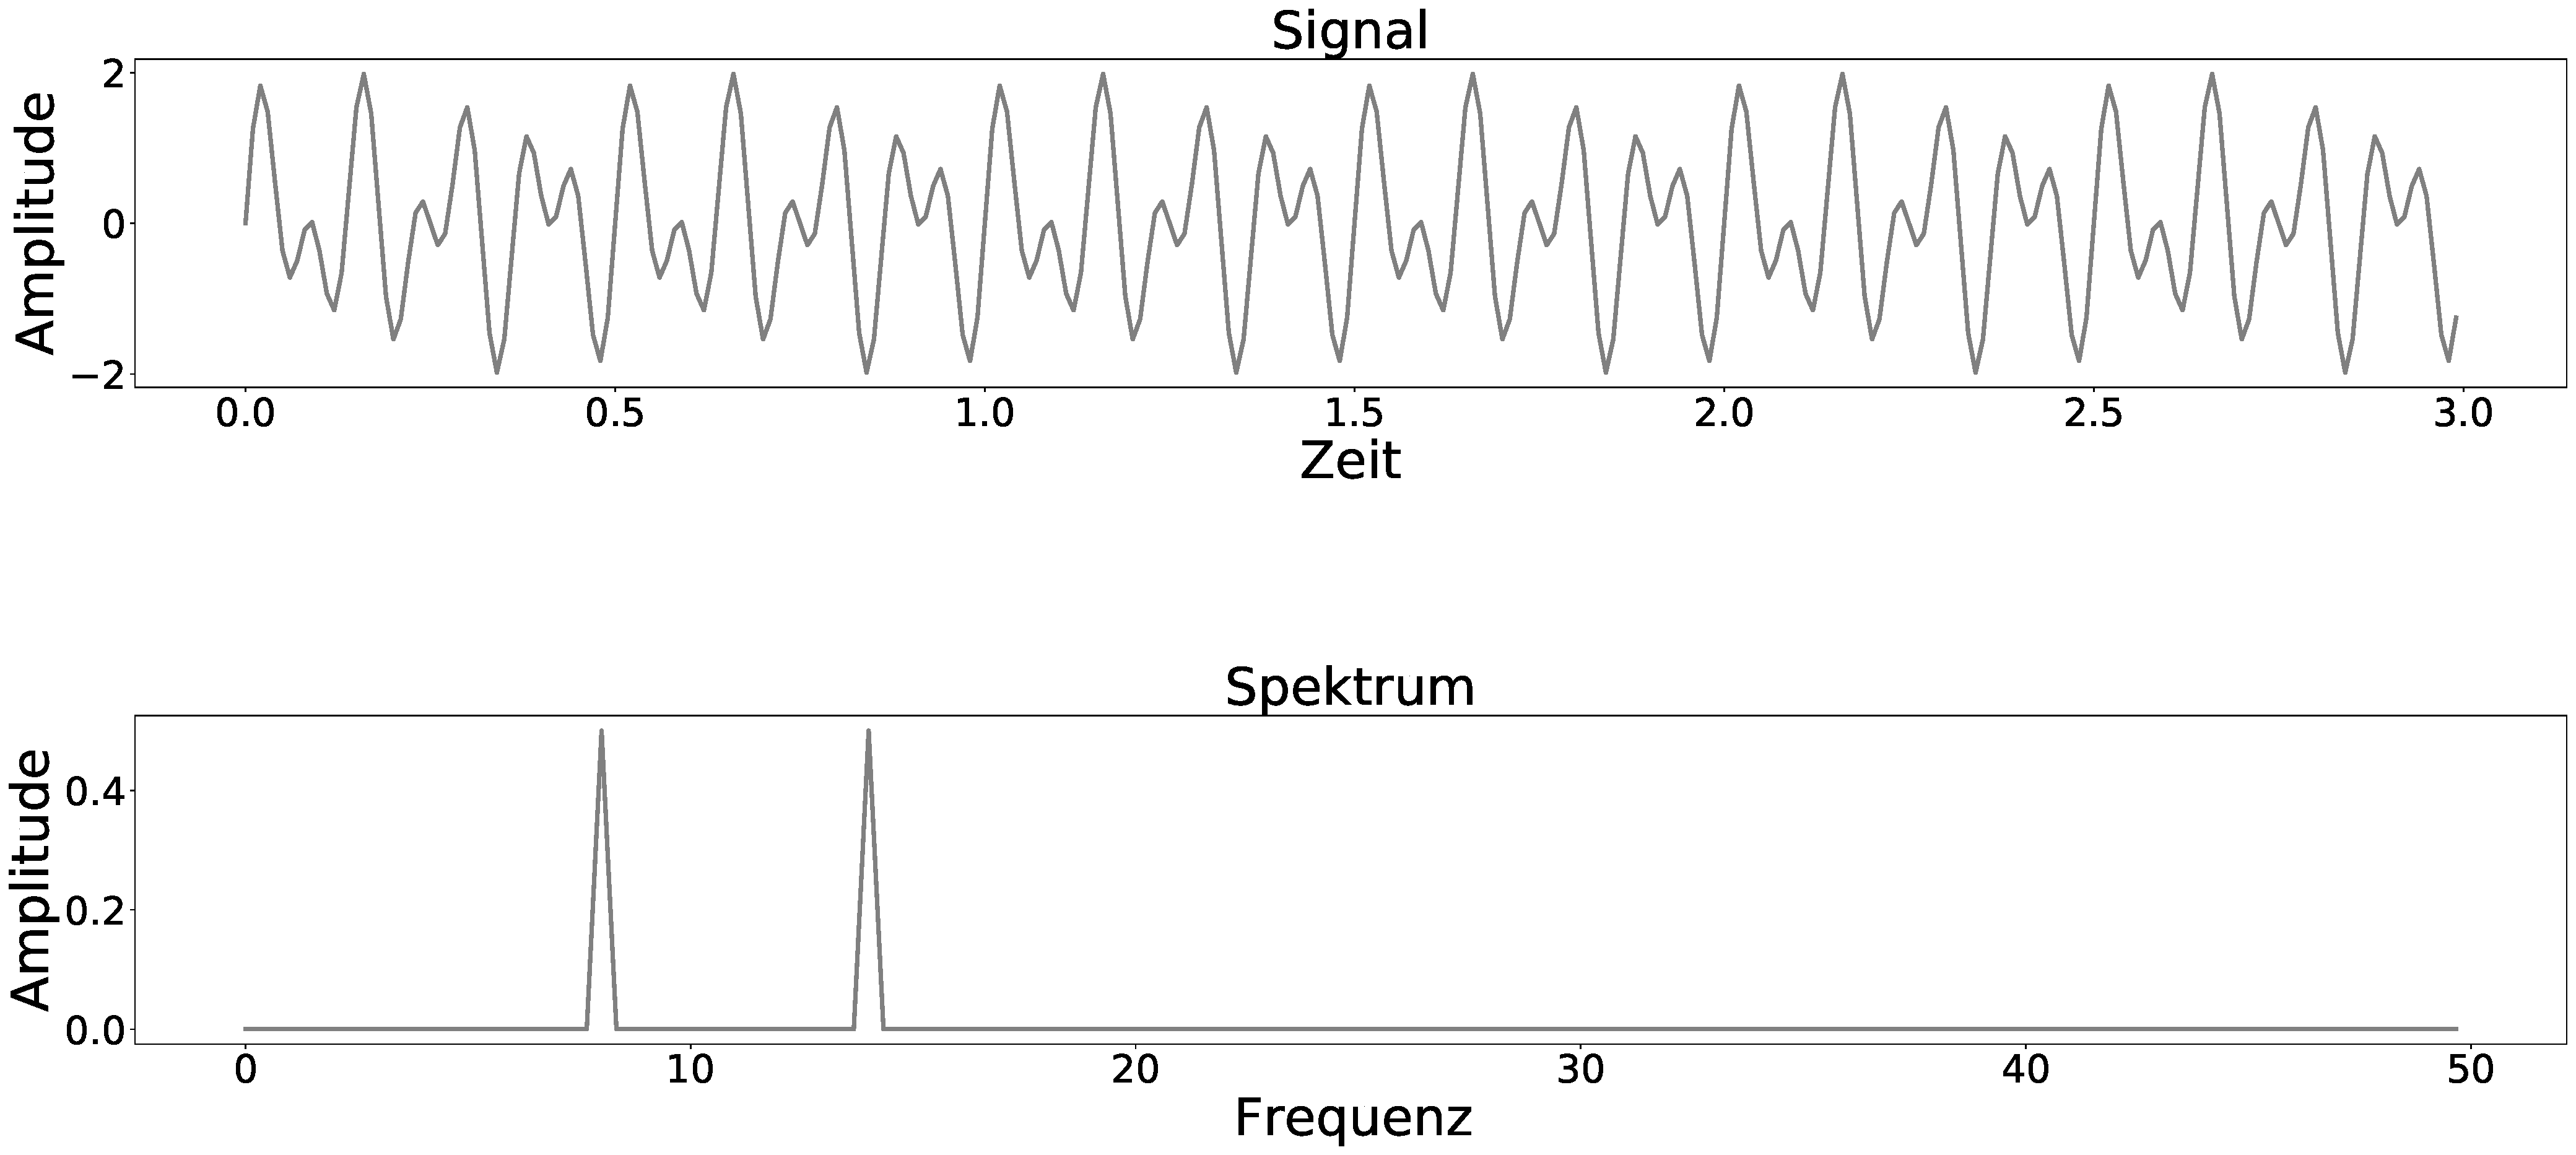
\includegraphics[width=1\textwidth]{attachments/fft_example.pdf}
    \caption[Aufspaltung eines Signals in dessen Frequenzteile]{Aufspaltung eines Signals in dessen Frequenzteile (eigene Darstellung)}
    \label{fig:aufspaltung_eines_Signals_in_dessen_Frequenzteile}
\end{figure}

Bei der Berechnung einer \ac{dft} steigt dessen Komplexität $O$ mit der Anzahl der Abtastpunkte $N$ quadratisch an, wie in der \autoref{form:berechnung_der_dft_komplexitaet} dargestellt.
Dies führt bei hohen Samplegrößen zu einer extremen Rechenzeit, was nicht praktikabel ist \autocite{fft:002}.

\begin{equ}[ht!]
    \begin{equation}
        O(N) = N^2
    \end{equation}
    \caption[Berechnung der \ac{dft}-Komplexität]{Berechnung der \ac{dft}-Komplexität \autocite{fft:002}}
    \label{form:berechnung_der_dft_komplexitaet}
\end{equ}


Im Gegensatz zur \ac{dft} stellt die \ac{fft} ein Algorithmus dar, mit welchem der Rechenaufwand deutlich reduziert wird.
Aus diesem Grund wird häufig die \ac{fft} genutzt, welche nach dem 'Teile und Herrsche'-Verfahren funktioniert und nur noch eine Komplexität von $O(N) = (N \: log(N))$ besitzt \autocite{fft:002}.
Durch diese enorme Zeit- und Rechenersparnis findet die \ac{fft} in vielen Bereichen, wie z.B. in Ingenieurswissenschaften, Musik, der Wissenschaft und der Mathematik Verwendung \autocite{wiki:010}.
Für die Berechnung der \ac{fft} sind mehrere Algorithmen verfügbar, wobei in dieser Masterarbeit der Radix-2 Algorithmus von der \ac{cmsis}-\ac{dsp} Bibliothek verwendet wurde.

\clearpage 

Als Vorraussetzung des Algorithmus der \ac{fft} muss die Anzahl der Messwerte $N$, auch Samples genannt, einer Zweierpotenz entsprechen \autocite{fft:002}.

\begin{equ}[ht!]
    \begin{equation}
        N = 2^N, N \in \mathbb{N}
    \end{equation}
    \begin{center}
        \begin{tabular}{lcr}
            $N$ & Anzahl von Samples \\
            $\mathbb{N}$ & natürliche Zahlen\\
        \end{tabular}
    \end{center}
    \caption[Rechenbedingung der \ac{fft}]{Rechenbedingung der \ac{fft} \autocite{fft:002}}
    \label{form:rechenbedingung_der_fft}
\end{equ}

Wird die Rechenbedingung in \autoref{form:rechenbedingung_der_fft} erfüllt, kann, wie in \autoref{form:aufteilung_der_dft} zu sehen, diese in zwei Teilsummen zerlegt werden, je eine für gerade und ungerade Indizes.

\begin{equ}[ht!]
    \begin{equation}
        X(k) = \sum_{n=0}^{N-1} x(n) \: w_N^{n \: k} = \sum_{n=0,2,...}^{N-2} x(n) \: w_N^{n \: k} +  \sum_{n=1,3,...}^{N-1} x(n) \: w_N^{n \: k}
    \end{equation}
    \begin{center}
        \begin{tabular}{lcr}
            $w = e ^ {-j \: \frac{2 \: \pi}{N}}$ & komplexer Drehfaktor der \ac{dft} \\
        \end{tabular}
    \end{center}
    \caption[Aufteilung der \ac{dft}]{Aufteilung der \ac{dft} (\ac{iaa} \cite{fft:002})}
    \label{form:aufteilung_der_dft}
\end{equ}

Anschließend wird eine Substitution wie in \autoref{form:substitution_der_dft} zu sehen, angewandt.

\begin{table}[ht!]
    \begin{center}
        \begin{tabular}{lcr}
            $n = 2m$ & für $n$ gerade \\
            $n = 2m + 1$ & für $n$ ungerade \\
            $M = N / 2$ & als Abkürzung 
        \end{tabular}
    \end{center}
    \caption[Substitution der \ac{dft}]{Substitution der \ac{dft} (\ac{iaa} \cite{fft:002})}
    \label{form:substitution_der_dft}
\end{table}

Unter Berücksichtigung der Umformungen aus \autoref{form:umformung_dft} resultieren zwei Formeln mit der halben Länge, wie in \autoref{form:resultierende_gleichungen_nach_der_Aufspaltung_der_dft} dargestellt.
\begin{equ}[ht!]
    \begin{equation}
        w_N^{2m \: k} = w_M^{m \: k} \qquad \text{und}\qquad w_N^{(2m + 1) \: k} = w_N^k \: w_M^{m \: k}
    \end{equation}
    \caption[Umformung \ac{dft}]{Umformung \ac{dft} (\ac{iaa} \cite{fft:002})}
    \label{form:umformung_dft}
\end{equ}

\begin{equ}[H]
    \begin{equation}
        X(k) = \sum_{m=0}^{M-1} x(2m) \: w_M^{m \: k} + \sum_{m=0}^{M-1} x(2m + 1) \: w_M^{m \: k}
    \end{equation}
    \caption[Resultierende Formeln nach Aufspaltung der \ac{dft}]{Resultierende Gleichungen nach Aufspaltung der \ac{dft} (\ac{iaa} \cite{fft:002})}
    \label{form:resultierende_gleichungen_nach_der_Aufspaltung_der_dft}
\end{equ}
Ist die resultierende Länge der \ac{dft} wieder eine Zweierpotenz, wird die Zerlegung solange fortgeführt, bis $N$ Vektoren der Länge $2^0$ erhält \autocite{fft:002}.
Anschließend werden die Ergebnisse zusammengerechnet und die \ac{dft} wurde gelöst \autocite{fft:002}.
\end{document}


